\documentclass[12pt]{article}
\usepackage[hidelinks]{hyperref}
%\documentclass[journal,12pt,twocolumn]{IEEEtran}
\usepackage[none]{hyphenat}
\usepackage{graphicx}
\usepackage{listings}
\usepackage[english]{babel}
\usepackage{graphicx}
\usepackage{siunitx}
\usepackage{caption}
\usepackage{hyperref}
\usepackage{booktabs}
\def\inputGnumericTable{}
\usepackage{color}
\usepackage{array}
\usepackage{longtable}
\usepackage{calc}
\usepackage{multirow}
\usepackage{hhline}
\usepackage{ifthen}
\usepackage{array}
\usepackage{listings}
\usepackage{caption}
\usepackage{refstyle}
\usepackage{amssymb} % for \because
\usepackage{amsmath}   % for having text in math mode
\usepackage{extarrows} % for Row operations arrows
\usepackage{listings}
\graphicspath{{/storage/self/primary/Download/codes/math/9/tables}}
\usepackage[utf8]{inputenc}
\lstset{
language=tex,
frame=single, 
breaklines=true
}
\usepackage{hyperref}
  
%Following 2 lines were added to remove the blank page at the beginning
\usepackage{atbegshi}% http://ctan.org/pkg/atbegshi
\AtBeginDocument{\AtBeginShipoutNext{\AtBeginShipoutDiscard}}
\usepackage{setspace}
\usepackage{gensymb}
\usepackage{xcolor}
\singlespacing
\usepackage{siunitx}
\usepackage{amsmath}
\usepackage{mathtools}
\usepackage{hyperref}
\usepackage{amsthm}
\usepackage{mathrsfs}
\usepackage{txfonts}
\usepackage{stfloats}
\usepackage{cite}
\usepackage{cases}
\usepackage{subfig}
\usepackage{longtable}
\usepackage{multirow}
\usepackage{enumitem}
\usepackage{mathtools}
\usepackage{listings}
\usepackage{tikz}
\usetikzlibrary{shapes,arrows,positioning}
\usepackage{circuitikz}
\let\vec\mathbf
\DeclareMathOperator*{\Res}{Res}
\graphicspath{{/sdcard/Download/vectors/figs}}
%Following 2 lines were added to remove the blank page at the beginning
\usepackage{atbegshi}% http://ctan.org/pkg/atbegshi
\AtBeginDocument{\AtBeginShipoutNext{\AtBeginShipoutDiscard}}
%



%New macro definitions
\newcommand{\mydet}[1]{\ensuremath{\begin{vmatrix}#1\end{vmatrix}}}
\providecommand{\brak}[1]{\ensuremath{\left(#1\right)}}
\providecommand{\norm}[1]{\left\lVert#1\right\rVert}
\newcommand{\solution}{\noindent \textbf{Solution: }}
\newcommand{\myvec}[1]{\ensuremath{\begin{pmatrix}#1\end{pmatrix}}}
\providecommand{\abs}[1]{\left\vert#1\right\vert}
\let\vec\mathbf{}
\begin{document}

\begin{center}
\title{\textbf{VECTORS}}
\date{\vspace{-5ex}} %Not to print date automatically
\maketitle
\end{center}
\setcounter{page}{1}
\section*{12$^{th}$ Maths - Chapter 10 - EXERCISE 5.9}

\begin{enumerate}

	\item Find the position vector of a point $\vec{R}$ which divides the line joining two points $\vec{ P}$ and $\vec{Q}$ whose position vectors are $\vec{P} = \myvec{2\\ 1 }$ and $\vec{Q} = \myvec{ 1\\-3 }$  externally in the ratio 1:2.Also show that $\vec{P}$ is the midpoint of the linesegment RQ.

\solution The input parameters for this problem are available in Table \ref{Table-1}
\begin{table}[ht!]
\begin{tabular}{|c|c|p{5cm}|}
\hline
\textbf{Symbol} & \textbf{Value} & \textbf{Description} \\
\hline
$\theta$ & $30\degree$ & $\angle{BAP} = \angle{BAQ}$ \\
\hline
$a$ & $9$ & $AB$ \\
\hline
$c$ & $8$ & $AQ$ \\
\hline
$\vec{e}_1$ & $\myvec{1\\0}$ & Basis vector \\
\hline
\end{tabular}

\caption{}
\label{Table-1}	
\end{table}
	
$\vec{R}$ divides the line joining two points $\vec{P}$ and $\vec{Q}$ 
\begin{align}
\vec{P} = \myvec{ 2\\1}
\label{eq:eq:1}\\ 
\vec{Q} = \myvec{ 1\\-3}
\end{align}
When $\vec{R}$ divides line segment joining $\vec{P}$ and $\vec{Q}$ externally,
\begin{align}
	\vec{R} &= \frac{1\vec{Q}-2\vec{P}}{-1}
	         = \myvec{3\\5}
\end{align}	
Also,
		Let the midpoint of $\vec{R}$ and $\vec{Q}$ be $\vec{P}$ , Position vector of $\vec{P}$ is given by
\begin{align}
	\vec{P} &= \frac{(\vec{R} + \vec{Q})}{2} 
	=\myvec{2\\1}
	\label{eq:eq:4}
\end{align}
		
			\eqref{eq:4} is same as \eqref{eq:1}
		
See Fig.
\ref{fig:/storage/self/primary/Download/codes/math/9/figs/figure1}.
\begin{figure}[!h]
	\begin{center}
	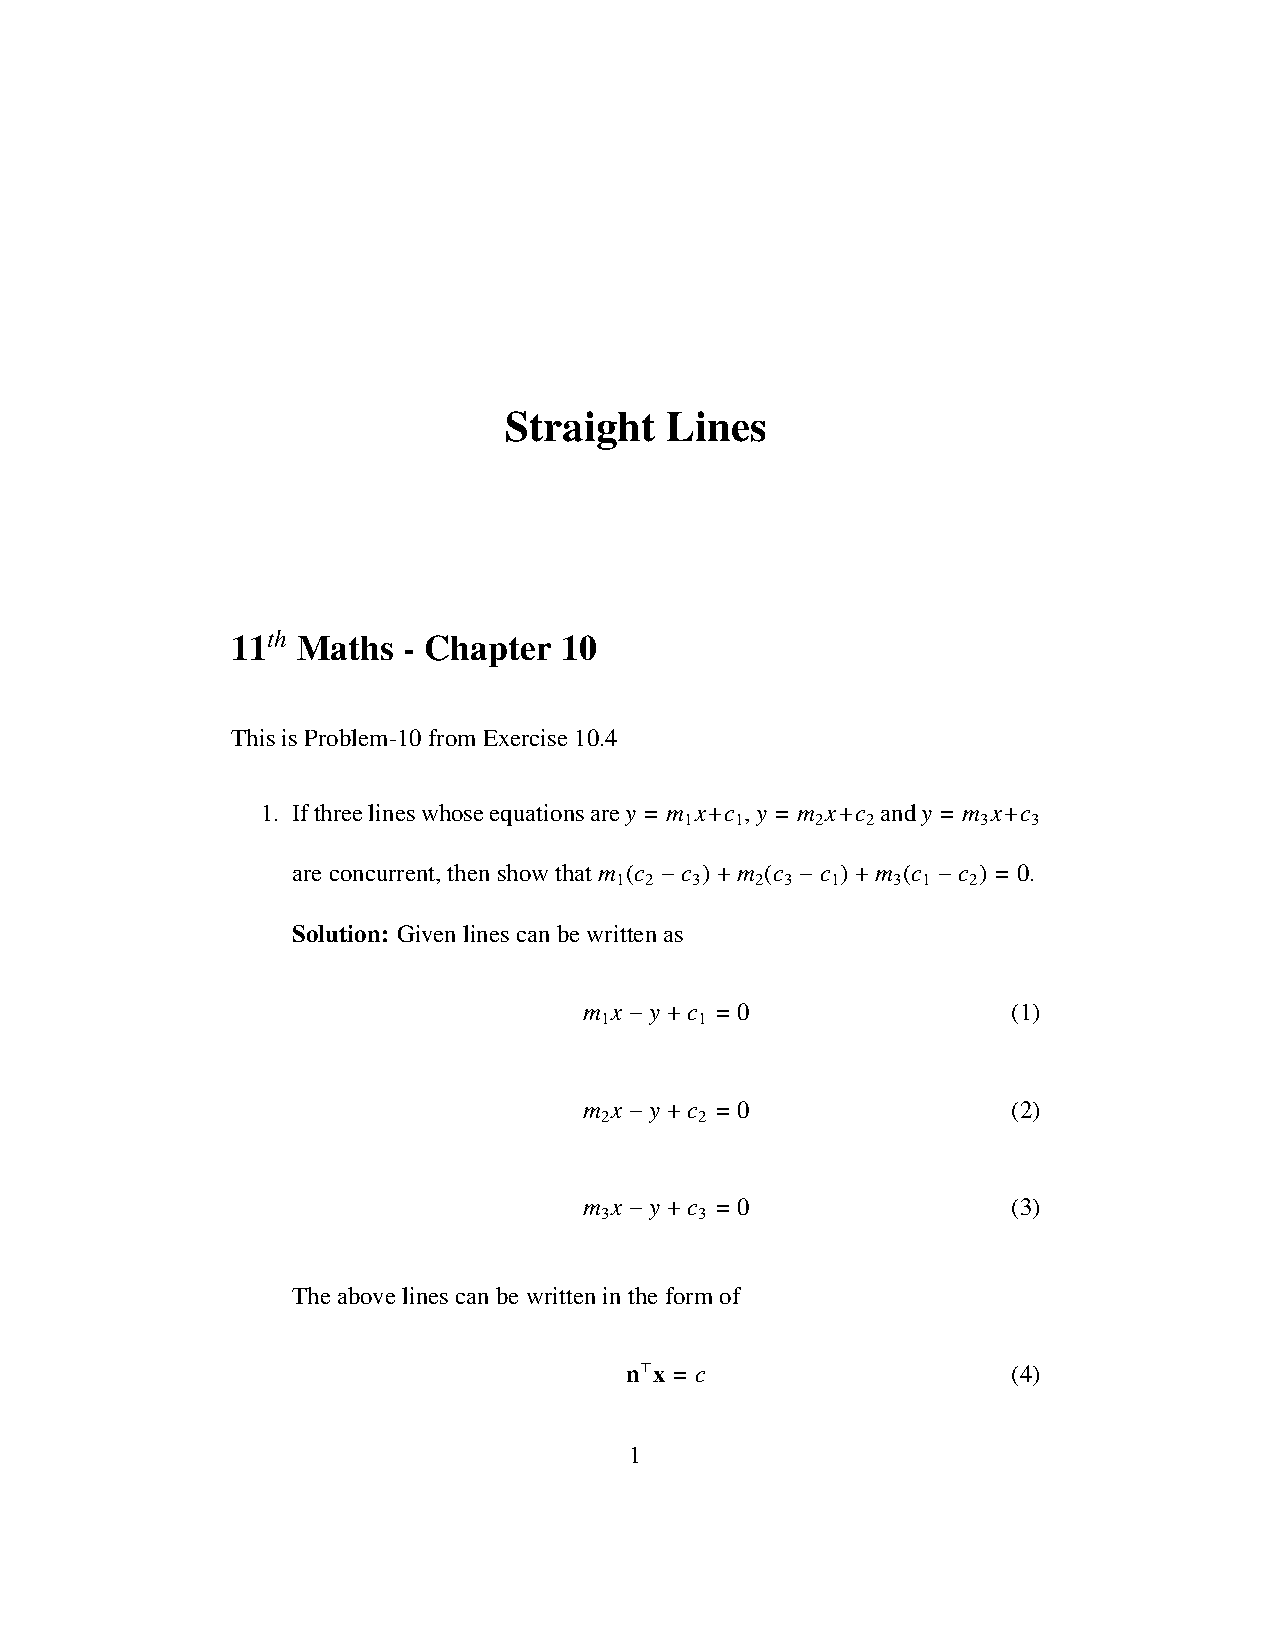
\includegraphics[width=\columnwidth]{/storage/self/primary/Download/codes/math/9/figs/line.png}
	\end{center}
        \caption{}
        \label{fig:/storage/self/primary/Download/codes/math/9/figs/figure1}
 \end{figure}
\end{enumerate}
\end{document}
